\begin{tabular}{M{6.5cm}M{11cm}}
	\textbf{TRUNG TÂM MANABIE}& \textbf{ĐỀ ÔN TẬP KIỂM TRA CUỐI HỌC KÌ 1}\\
	\textbf{MÃ ĐỀ: 003}& \textbf{Bài thi môn: VẬT LÝ 12}\\
	\textit{(Đề trường THPT Thuận Thành số 1 - Bắc Ninh năm học 2024 -2025)}& \textit{Thời gian làm bài: 50 phút, không kể thời gian phát đề}
	
	\noindent\rule{4cm}{0.8pt} \\
\end{tabular}
\setcounter{section}{0}
\section{Câu trắc nghiệm nhiều phương án lựa chọn}
\textit{Thí sinh trả lời từ câu 1 đến câu 18. Mỗi câu hỏi thí sinh chọn một phương án}
\setcounter{ex}{0}
\Opensolutionfile{ans}[ans/FINAL-SEM1-003-TN]
% ===================================================================
\begin{ex}
	Gọi $p$, $V$, $T$ và $n$ lần lượt là áp suất, thể tích, nhiệt độ và mật độ phân tử của một khối khí lí tuongr xác định. Khi làm nóng khối khí lí tưởng bằng quá trình đẳng áp thì tỉ số nào sau đây không đổi?
	\choice
	{$\dfrac{n}{T}$}
	{\True $\dfrac{V}{T}$}
	{$\dfrac{p}{T}$}
	{$\dfrac{n}{p}$}
	\loigiai{}
\end{ex}
% ===================================================================
\begin{ex}
	Sự chuyển thể nào sau đây xảy ra ở một nhiệt độ xác định dưới một áp suất cho trước?
	\choice
	{Ngưng tụ}
	{Thăng hoa}
	{\True Sôi}
	{Bay hơi}
	\loigiai{}
\end{ex}
% ===================================================================
\begin{ex}
	Biết nhiệt dung riêng của nước và rượu lần lượt là $\SI{4180}{\joule/\kilogram\cdot\kelvin}$ và $\SI{2500}{\joule/\kilogram\cdot\kelvin}$. Dùng một ấm điện có công suất không đổi lần lượt đun nóng cùng một khối lượng nước và rượu. Biết nhiệt độ ban đầu của nước và rượu bằng nhau. Nhận xét nào sau đây đúng?
	\choice
	{Nước nóng nhanh hơn rượu}
	{Ban đầu nước nóng nhanh hơn, lúc sau rượu nóng nhanh hơn}
	{\True Rượu nóng nhanh hơn nước}
	{Nước và rượu nóng nhanh như nhau}
	\loigiai{}
\end{ex}
% ===================================================================
\begin{ex}
	Một lượng khí lí tưởng chứa trong một xilanh có thể tích $\SI{10}{\liter}$ và áp suất $\SI{1.5}{atm}$. Sau khi nén đẳng nhiệt, thể tích giảm đi $\SI{6}{\liter}$. Áp suất của khí khi đó là
	\choice
	{\True $\SI{3.75}{atm}$}
	{$\SI{2.50}{atm}$}
	{$\SI{0.90}{atm}$}
	{$\SI{0.60}{atm}$}
	\loigiai{
		$p_1V_1=p_2V_2\Leftrightarrow 1,5\cdot10=6\cdotp_2\Rightarrow p_2=\SI{3.75}{atm}$.
	}
\end{ex}
% ===================================================================
\begin{ex}
	Tính chất nào sau đây không phải của chất ở thể khí?
	\choice
	{Hình dạng thay đổi theo bình chứa}
	{Gây áp suất lên thành bình chứa theo mọi hướng}
	{Các phân tử chuyển động hỗn loạn không ngừng}
	{\True Khó nén hơn so với thể lỏng}
	\loigiai{}
\end{ex}
% ===================================================================
\begin{ex}
	Khi một vật có nhiệt độ ở "Độ không tuyệt đối" thì
	\choice
	{động năng của các phân tử cực đại}
	{thế năng tương tác giữa các phân tử bằng không}
	{thế năng tương tác giữa các phân tử cực đại}
	{\True động năng của các phân tử bằng không}
	\loigiai{}
\end{ex}
% ===================================================================
\begin{ex}
	Người ta thực hiện công $\SI{120}{\joule}$ để nén khí trong một xilanh. Khối khí truyền ra môi trường xung quanh nhiệt lượng $\SI{30}{\joule}$. Nội năng của khối khí
	\choice
	{tăng $\SI{150}{\joule}$}
	{giảm $\SI{90}{\joule}$}
	{\True tăng $\SI{90}{\joule}$}
	{giảm $\SI{150}{\joule}$}
	\loigiai{
		$\Delta U=A+Q=120-30=\SI{90}{\joule}$.
	}
\end{ex}
% ===================================================================
\begin{ex}
	Tại sao các phân tử khí có thể chuyển động tự do trong không gian?
	\choice
	{Do lực hút giữa các phân tử khí rất mạnh}
	{Do các phân tử khí có khối lượng rất nhỏ}
	{\True Do lực hút giữa các phân tử khí rất yếu}
	{Do các phân tử khí luôn đẩy nhau}
	\loigiai{}
\end{ex}
% ===================================================================
\begin{ex}
	Cồn y tế chuyển từ thể lỏng sang thể khí rất nhanh ở điều kiện thông thường. Khi xoa cồn vào da, ta cảm thấy lạnh ở vùng da đó vì cồn
	\choice
	{\True thu nhiệt lượng từ cơ thể qua chỗ da đó để bay hơi}
	{khi bay hơi tỏa nhiệt lượng vào chỗ da đó}
	{khi bay hơi kéo theo lượng nước chỗ da đó ra khỏi cơ thể}
	{khi bay hơi tạo ra dòng nước mát tại chỗ da đó}
	\loigiai{}
\end{ex}
% ===================================================================
\begin{ex}
	Một khối chất rắn kết tinh có khối lượng $m$ và nhiệt nóng chảy riêng $\lambda$. Ở nhiệt độ nóng chảy, nhiệt lượng cần cung cấp để khối chất nóng chảy hoàn toàn là
	\choice
	{$Q=\dfrac{m}{\lambda}$}
	{$Q=\dfrac{1}{m\lambda}$}
	{\True $Q=\lambda m$}
	{$Q=\dfrac{\lambda}{m}$}
	\loigiai{}
\end{ex}
% ===================================================================
\begin{ex}
	\immini{Một áp kế gồm một bình cầu thủy tinh có thể tích $V_0$ gắn với một ống nhỏ nằm ngang tiết diện ống là $\SI{0.1}{\centi\meter^2}$. Biết ở $\SI{10}{\celsius}$ và $\SI{20}{\celsius}$, giọt thủy ngân cách thành bình lần lượt là $d_1=\SI{10}{\centi\meter}$ và $d_2=\SI{140}{\centi\meter}$. Dung tích của bình cầu là	}
	{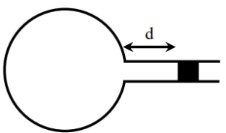
\includegraphics[scale=0.6]{../figs/FINAL-SEM1-003-1}}
	\choice
	{\True $\SI{366.9}{\centi\meter^3}$}
	{$\SI{36.69}{\centi\meter^3}$}
	{$\SI{32.43}{\centi\meter^3}$}
	{$\SI{324.3}{\centi\meter^3}$}
	\loigiai{
		Đẳng áp $\dfrac{V_1}{T_1}=\dfrac{V_2}{T_2}\Leftrightarrow\dfrac{V_c+Sd_1}{T_1}=\dfrac{V_c+Sd_2}{T_2}\Rightarrow\dfrac{V_c+0,1\cdot10}{10+273}=\dfrac{V_c+0,1\cdot140}{20+273}\Rightarrow V_c=\SI{366.9}{\centi\meter^3}$.
	}
\end{ex}
% ===================================================================
\begin{ex}
	\immini{Biển báo sau đây cảnh báo điều gì?	
		\choice
		{Nơi có nhiều gió}
		{\True Nơi có chất phóng xạ}
		{Nơi có nhiệt độ cao}
		{Vật liệu dễ bay hơi}}
	{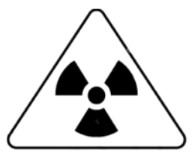
\includegraphics[scale=0.6]{../figs/FINAL-SEM1-003-2}}
	\loigiai{}
\end{ex}
% ===================================================================
\begin{ex}
	Đặc điểm nào sau đây là đúng với cấu trúc của chất ở thể lỏng?
	\choice
	{Các phân tử có lực tương tác rất yếu}
	{Các phân tử chuyển động hỗn loạn và có khoảng cách rất lớn}
	{Giữa các phân tử không có khoảng cách}
	{\True Các phân tử dao động quanh vị trí cân bằng, vị trí cân bằng có thể dịch chuyển}
	\loigiai{}
\end{ex}
% ===================================================================
\begin{ex}
	Trong quá trình biến đổi đẳng nhiệt của khí lí tưởng thì	
	\choice
	{nội năng của khí tăng}
	{nội năng của khí giảm}
	{\True nội năng của khí không đổi}
	{khí không thực hiện công}
	\loigiai{
		Nội năng của khí lí tưởng chỉ phụ thuộc nhiệt độ nên trong quá trình biến đổi đẳng nhiệt thì nội năng của khí lí tưởng không đổi.
	}
\end{ex}
% ===================================================================
\begin{ex}
	\immini{Trên hình bên là hai đường đẳng nhiệt của cùng một lượng khí lí tưởng ở hai nhiệt độ khác nhau. Thông tin đúng khi so sánh nhiệt độ $T_1$ và $T_2$ là 
		\choice
		{$T_2<T_1$}
		{\True $T_2>T_1$}
		{$T_2=2T_1$}
		{$T_2=T_1$}}
	{\vspace{-1cm}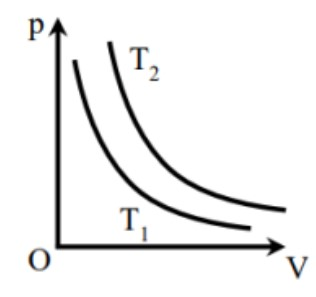
\includegraphics[scale=0.6]{../figs/FINAL-SEM1-003-3}}
	\loigiai{}
\end{ex}
% ===================================================================
\begin{ex}
	Một khối khí trong một xi lanh kín nhận được nhiệt lượng $Q$ và sinh công $A$. Trong hệ thức của định luật I nhiệt động lực học $\Delta U=A+Q$, $Q$ và $A$ phải có quy ước dấu nào sau đây?
	\choice
	{$Q<0$ và $A>0$}
	{$Q<0$ và $A<0$}
	{$Q>0$ và $A>0$}
	{\True $Q>0$ và $A<0$}
	\loigiai{}
\end{ex}
% ===================================================================
\begin{ex}
	Laser (Laze) được sử dụng để khoan kim loại vì nó có thể tạo ra một chùm tia sáng với năng lượng lớn, tập trung vào một điểm nhỏ và có độ chính xác cao. Dùng một mũi khoan laser có công suất $\SI{200}{\watt}$ để khoan vào một khối kim loại. Biết nhiệt nóng chảy riêng của kim loại là $\SI{250}{\joule/\gram}$, khối lượng riêng của kim loại là $\SI{7.8}{\gram/\centi\meter^3}$ và đường kính mũi khoan là $\SI{0.2}{\centi\meter}$. Giả sử đã nung nóng kim loại đến nhiệt độ nóng chảy để khoan. Lấy $\pi=3,14$. Thời gian tối thiểu để khoan qua một lỗ tròn có độ dày $\SI{0.5}{\centi\meter}$ là bao nhiêu?
	\choice
	{$\SI{0.252}{\second}$}
	{$\SI{0.604}{\second}$}
	{$\SI{0.323}{\second}$}
	{\True $\SI{0.153}{\second}$}
	\loigiai{
		$V=\pi \cdot\dfrac{d^2}{4}\cdot h=\xsi{0,005\pi}{\centi\meter^3}$.\\
		$m=\rho V=\xsi{0,039\pi}{\gram}$.\\
		$t=\dfrac{Q}{\calP}=\dfrac{m\lambda}{\calP}\approx\SI{0.153}{\second}$.
	}
\end{ex}
% ===================================================================
\begin{ex}
Theo thang nhiệt độ Celsius, nhiệt kế y tế đo được nhiệt độ từ $\SI{35}{\celsius}$ đến $\SI{42}{\celsius}$. Nếu tính theo thang nhiệt độ Kelvin thì nhiệt kế này đo được nhiệt độ	
	\choice
	{\True từ $\SI{308}{\kelvin}$ đến $\SI{315}{\kelvin}$}
	{từ $\SI{135}{\kelvin}$ đến $\SI{142}{\kelvin}$}
	{từ $\SI{231}{\kelvin}$ đến $\SI{315}{\kelvin}$}
	{từ $\SI{238}{\kelvin}$ đến $\SI{308}{\kelvin}$}
	\loigiai{}
\end{ex}
\Closesolutionfile{ans}
\section{Câu trắc nghiệm đúng/sai} 
\textit{Thí sinh trả lời từ câu 1 đến câu 4. Trong mỗi ý \textbf{a)}, \textbf{b)}, \textbf{c)}, \textbf{d)} ở mỗi câu, thí sinh chọn đúng hoặc sai}
\setcounter{ex}{0}
\Opensolutionfile{ans}[ans/FINAL-SEM1-003-TF]
% ===================================================================
\begin{ex}
	\immini{Một hệ làm nóng nước bằng năng lượng mặt trời có hiệu suất chuyển đổi $\SI{22}{\percent}$, cường độ bức xạ mặt trời lên bộ thu nhiệt là $\SI{980}{\watt/\meter^2}$, diện tích bộ thu là $\SI{20}{\meter^2}$. Cho nhiệt dung riêng của nước là $\SI{4180}{\joule/\kilogram\cdot\kelvin}$, khối lượng riêng của nước là $\SI{1000}{\kilogram/\meter^3}$.}
	{\vspace{-0.75cm}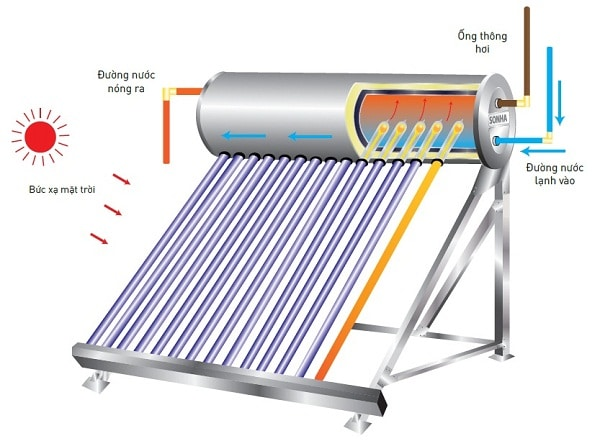
\includegraphics[scale=0.2]{../figs/FINAL-SEM1-003-4}}
	\choiceTF[t]
	{Công suất bức xạ chiếu lên bộ thu nhiệt là $\SI{20}{\kilo\watt}$}
	{\True Hệ thống thu nhiệt nhận được $\SI{100}{\joule}$ năng lượng mặt trời thì nội năng của nước tăng thêm $\SI{22}{\joule}$}
	{\True Trong 30 phút, năng lượng mặt trời chiếu lên bộ thu nhiệt là $\SI{35.28}{\mega\joule}$}
	{\True Nếu hệ thống đó làm nóng 40 lít nước thì trong khoảng thời gian 30 phút, nhiệt độ của nước tăng thêm $\SI{46.4}{\celsius}$}
	\loigiai{\begin{itemchoice}
			\itemch Sai. $\calP=IS=\SI{19.6}{\kilo\watt}$.
			\itemch Đúng.
			\itemch Đúng.
			\itemch Đúng.
	\end{itemchoice}}
\end{ex}
% ===================================================================
\begin{ex}
	\immini{Một xilanh có pittông rất nhẹ, bên trong chứa một lượng khí có thể tích ban đầu $\SI{500}{\centi\meter^3}$. Biết diện tích của pittông là $\SI{50}{\centi\meter^2}$. Áp suất khí quyển là $p_0=\SI{E5}{\pascal}$. Xem nhiệt độ khối khí không đổi, bỏ qua ma sát giữa pittông và thành xilanh. Lấy $g=\SI{10}{\meter/\second^2}$.}
	{\vspace{-0.75cm}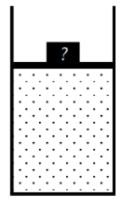
\includegraphics[scale=0.7]{../figs/FINAL-SEM1-003-5}}
	\choiceTF[t]
	{\True Ban đầu chiều cao cột khí trong xilanh là $\SI{10}{\centi\meter}$}
	{Đặt lên pittông một quả cân khối lượng $m$ thì pittông dịch chuyển xuống một đoạn $\xsi{x}{\centi\meter}$, khi đó áp suất khí giảm}
	{Đặt lên pittông một quả cân có khối lượng $\SI{10}{\kilogram}$ thì pittông dịch chuyển xuống dưới một đoạn $\SI{1.5}{\centi\meter}$}
	{\True Khối khí đang ở trạng thái cân bằng như khi có thêm quả cân $\SI{10}{\kilogram}$ đặt lên pittông, nếu cung cấp cho khối khí nhiệt lượng $\SI{150}{\joule}$, khối khí trở về thể tích ban đầu $\SI{500}{\centi\meter^3}$. Trong quá trình đó áp suất khí không đổi. Độ biến thiên nội năng của khối khí khi đó là $\SI{140}{\joule}$}
	\loigiai{\begin{itemchoice}
			\itemch Đúng.
			\itemch Sai.\\
			$p=p_0+\dfrac{mg}{S}=\SI{1.2E5}{\pascal}$.
			\itemch Sai.\\
			$p_0S\ell_0=pS\ell\Leftrightarrow 10^5\cdot10=1,2\cdot10^5\cdot\ell\Rightarrow \ell=\xsi{\dfrac{25}{3}}{\centi\meter}$.\\
			$x=\ell_0-\ell\approx\SI{1.67}{\centi\meter}$.
			\itemch Đúng.
	\end{itemchoice}}
\end{ex}
% ===================================================================
\begin{ex}
\immini{Có thể sử dụng bộ dụng cụ thí nghiệm như hình bên để tìm hiểu mối liên hệ giữa thể tích và nhiệt độ của một lượng khí xác định khi áp suất không đổi.}
{\vspace{-0.75cm}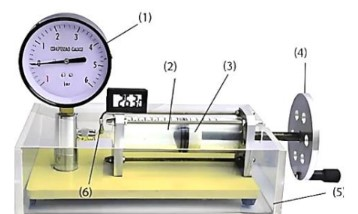
\includegraphics[scale=0.8]{../figs/FINAL-SEM1-003-6}}
\begin{center}
	\begin{tabular}{|M{2cm}|M{7cm}|M{7cm}|}
	\hline
	\thead{Lần đo} &\thead{Nhiệt độ khí trong xilanh\\
	$\xsi{t}{\left(\si{\celsius}\right)}$}&\thead{Thể tích khí trong xilanh\\
	$\xsi{V}{\left(\milli\liter\right)}$}\\
	\hline
	1 & 45 & 75\\
	\hline
	2 & 41 & 74\\
	\hline
	3 & 37 & 73\\
	\hline
	4 & 32 & 72\\
	\hline
	5 & 28 & 71\\
	\hline
	\end{tabular}
\end{center}
	\choiceTF[t]
	{\True Khối khí trong xilanh gần đúng với khí lí tưởng}
	{\True Trình tự thí nghiệm: Nén và giữ áp suất của khí trong xilanh không đổi, ghi lại các giá trị của thể tích và nhiệt độ của khí trong xilanh, lặp lại các thao tác}
	{\True Với kết quả thí nghiệm thu được ở bảng trên, công thức liên hệ giữa thể tích và nhiệt độ tuyệt đối là $V/T=\SI{236E-3}{}$ ($V$ đo bằng $\si{\milli\liter}$)}
	{Biết áp suất của khí trong xi lanh là $\SI{E5}{\pascal}$, số phân tử khí trong xilanh là $\SI{1.71E24}{}$}
	\loigiai{\begin{itemchoice}
			\itemch Đúng.
			\itemch Đúng.
			\itemch Đúng. 
			\itemch Sai.\\
			$pV=\dfrac{N}{N_A}RT\Rightarrow N\approx\SI{1.71E21}{}$.
	\end{itemchoice}}
\end{ex}
% ===================================================================
\begin{ex}
\immini{Sinh viên thế hệ 8 X (những người sinh ra trong thập niên 1980) thường dùng "sục điện" để đun nước. Vào thời kỷ đó, hầu hết sinh viên đều có điều kiện kinh tế hạn chế, nên việc sắm một chiếc ấm đun nước điện là khá tốn kém. Sục điện là một lựa chọn vừa rẻ tiền, nhỏ gọn, linh hoạt, tiện dụng và đặc biệt tiết kiệm thời gian. Một đầu sục điện là một sợi kim loại xoắn kép - thường là nhôm, nối giữa hai đầu dây nhôm là đây điện có phích cắm. Lúc đun thì thả cái lõi kim loại đó vào trong cốc nhựa, xô nhựa chứa nước rồi cắm điện.}
{\vspace{-0.5cm}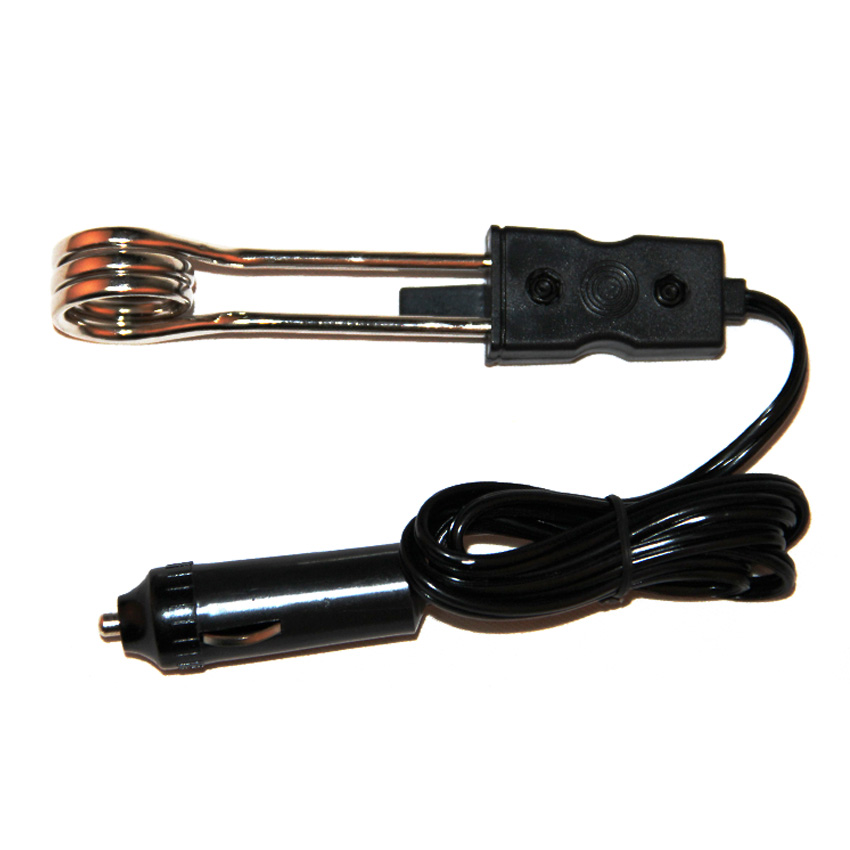
\includegraphics[scale=0.3]{../figs/FINAL-SEM1-003-7}}
Một sinh viên dùng chiếc sục điện có ghi $\SI{2500}{\watt}-\SI{220}{\volt}$ để đun 10 lít nước ở $\SI{20}{\celsius}$ chứa trong một xô nhựa. Ổ điện cắm sục có hiệu điện thế là $\SI{220}{\volt}$. Nước thu được $\SI{90}{\percent}$ nhiệt do dây xoắn kép tỏa ra. Biết khối lượng riêng của nước là $\SI{1000}{\kilogram/\meter^3}$, nhiệt dung riêng của nước là $\SI{4200}{\joule/\kilogram\cdot\kelvin}$. Nhiệt độ sôi của nước là $\SI{100}{\celsius}$.	
	\choiceTF[t]
	{\True Thiết bị này đã biến đổi trực tiếp điện năng thành nhiệt năng}
	{Để đun nước trong xô đến sôi, sinh viên đó cần đun trong 20,2 phút}
	{Muốn có nước tắm ở $\SI{40}{\celsius}$, sinh viên đó cần pha thêm 40 lít nước ở $\SI{20}{\celsius}$ vào 10 lít nước sôi}
	{Đây là thiết bị đun nước rất an toàn và đảm bảo sức khỏe nên được sinh viên chọn dùng phổ biến}
	\loigiai{\begin{itemchoice}
			\itemch Đúng.
			\itemch Sai. \\
			$Q=mc\Delta t=\rho Vc\Delta t=\SI{3.36E6}{\joule}$.\\
			$A=\dfrac{Q}{H}\approx\SI{3.73E6}{\joule}$.\\
			$t=\dfrac{A}{\calP}\approx\SI{24.9}{\minute}$.
			\itemch Sai. $t_{\text{cb}}=\dfrac{m_st_s+m_lt_l}{m_s+m_l}=\SI{36}{\celsius}$.
			\itemch Sai. Nguy cơ điện giật cao.
	\end{itemchoice}}
\end{ex}
\Closesolutionfile{ans}
\section{Câu trắc nghiệm trả lời ngắn} \textit{Thí sinh trả lời từ câu 1 đến câu 6}
\setcounter{ex}{0}
\Opensolutionfile{ans}[ans/FINAL-SEM1-003-TL]
% ===============================================================
\begin{ex}
	Một thợ rèn nhúng một con dao bằng thép có khối lượng $\SI{1.1}{\kilogram}$ ở nhiệt độ $\SI{850}{\celsius}$ vào trong bể nước lạnh để làm tăng độ cứng của lưỡi dao. Nước trong bể có thể tích 50 lít và có nhiệt độ bằng với nhiệt độ ngoài trời là $\SI{27}{\celsius}$. Bỏ qua sự truyền nhiệt cho thành bể và môi trường. Biết nhiệt dung riêng của thép là $\SI{460}{\joule/\kilogram\cdot\kelvin}$, của nước là $\SI{4200}{\joule/\kilogram\cdot\kelvin}$; khối lượng riêng của nước là $\SI{1}{\kilogram/\liter}$. Nhiệt độ của nước là bao nhiêu $\si{\celsius}$ khi có sự cân bằng nhiệt? (Kết quả được làm tròn đến chữ số hàng đơn vị)
	\shortans[oly]{29}
	\loigiai{
		
	}
\end{ex}
% ===============================================================
\begin{ex}
	Trong một xilanh chứa một lượng khí có áp suất $p=\SI{100}{\newton/\meter^2}$ thể tích $V_1=\SI{4}{\meter^3}$, nhiệt độ $t_1=\SI{57}{\celsius}$ được nung nóng đẳng áp đến nhiệt độ $t_2=\SI{87}{\celsius}$. Khí dãn nở đẩy pit-tông dịch chuyển đều. Biết nội năng của khối khí tăng thêm $\SI{100}{\joule}$. Nhiệt lượng đã truyền cho khối khí bằng cách nung nóng bằng bao nhiêu $\si{\joule}$? (Kết quả được làm tròn đến chữ số hàng đơn vị)
	\shortans[oly]{136}
	\loigiai{
		Qúa trình biến đổi trạng thái của khí trong xilanh là đẳng áp nên:
		$$\dfrac{V_2}{T_2}=\dfrac{V_1}{T_1}\Rightarrow V_2=\xsi{\dfrac{48}{11}}{\meter^3}.$$
		Công do khối khí thực hiện:
		$$A'=p\Delta V=\xsi{\dfrac{400}{11}}{\joule}.$$
	Nhiệt lượng đã truyền cho khối khí:
	$$Q=\Delta U-A=\Delta U+A'\approx\SI{136}{\joule}.$$
	}
\end{ex}
% ===============================================================
\begin{ex}
	Hô hấp ký là một kỹ thuật thăm dò chức năng hô hấp bằng cách đo thể tích thông khí mà bệnh nhân có thể hít vào và thở ra với gắng sức tối đa. Dùng để tầm soát, chẩn đoán và theo dõi những bệnh lý hô hấp như hen suyễn, bệnh phổi tắc nghẽn mãn tính. cũng như những tình trạng, bệnh lý hoặc thuốc có ảnh hưởng đến chức năng hồ hấp. Một bệnh nhân đến thăm khám tại bệnh viện và Bác sĩ sử dụng các kết quả hô hấp ký để xác định bạn có bị bệnh phổi tắc nghẽn mạn tính hay không và COPD nặng đến mức nào. Khi thở ra, dung tích của phổi là 2,50 lít và áp suất của không khí trong phổi là $\SI{101.75E3}{\pascal}$. Cho biết khi hít vào, áp suất này trở thành $\SI{101.04E3}{\pascal}$. Dung tích của phổi khi hít vào là bao nhiêu lít? Coi nhiệt độ khí trong phổi không đổi. (Kết quả làm tròn đến chữ số hàng phần trăm).
	\shortans[oly]{2,52}
	\loigiai{
		$pV=const\Rightarrow \SI{101.75E3}{}\cdot2,5=\SI{101.04E3}{}V\Rightarrow V\approx\SI{2.52}{\liter}$.
	}
\end{ex}
% ===============================================================
\begin{ex}
	Vận động viên chạy Marathon mất rất nhiều nước trong khi thi đấu. Các vận động viên thường chỉ có thể chuyển hóa khoảng $\SI{20}{\percent}$ năng lượng hóa học dự trữ trong cơ thể thành năng lượng dùng cho các hoạt động của cơ thể, đặc biệt là hoạt động chạy. Phần năng lượng còn lại chuyển thành nhiệt thải ra ngoài nhờ sự bay hơi của nước qua hô hấp và da để giữ cho nhiệt độ của cơ thể không đổi. Nếu vận động viên dùng hết $\SI{9}{\mega\joule}$ trong cuộc thi thì có khoảng bao nhiêu lít nước đã thoát ra khỏi cơ thể? Coi nhiệt độ cơ thể của vận động viên hoàn toàn không đổi và nhiệt hóa hơi riêng của nước trong cơ thể vận động viên là $\SI{2.45E6}{\joule/\kilogram}$. Lấy khối lượng riêng của mồ hôi là $\SI{1}{\kilogram/\liter}$. (Kết quả làm tròn đến chữ số hàng phần mười).
	\shortans[oly]{2,9}
	\loigiai{
		
	}
\end{ex}
% ===============================================================
\begin{ex}
	Trong một xilanh của động cơ đốt trong chứa một khối khí. Ban đầu khối khí có thể tích $\SI{4}{\deci\meter^3}$, áp suất $\SI{4}{atm}$ và nhiệt độ $\SI{47}{\celsius}$. Giai đoạn một: pittông nén xuống từ từ sao cho nhiệt độ khí không đổi, làm cho thể tích của khí còn $\SI{1}{\deci\meter^3}$. Sau đó, giai đoạn hai: khí được đun nóng, giãn nở đẩy pittông chuyển động lên làm thể tích khí tăng gấp 8 lần, áp suất khí luôn không đổi. Nhiệt độ cuối cùng của khối khí là bao nhiêu $\si{\celsius}$? (Kết quả được làm tròn đến chữ số hàng đơn vị)
	\shortans[oly]{2287}
	\loigiai{
		\begin{center}
			\begin{tabular}{|M{5cm}|M{5cm}|M{5cm}|}
				\hline
				$p$ & $V$ & $T$\\
				\hline
				$\SI{4}{atm}$ & $\SI{4}{\deci\meter^3}$ & $\SI{320}{\kelvin}$\\
				\hline
				$p$ & $\SI{1}{\deci\meter^3}$ & $\SI{320}{\kelvin}$\\
				\hline
				$p$ & $\SI{8}{\deci\meter^3}$ & $T_3$\\
				\hline
			\end{tabular}
		\end{center}
		$$\dfrac{V_2}{T_2}=\dfrac{V_3}{T_3}\Rightarrow\dfrac{1}{320}=\dfrac{8}{T_3}\Rightarrow T_3=\SI{2560}{\kelvin}\Rightarrow t_3\approx\SI{2287}{\celsius}.$$
	}
\end{ex}
% ===============================================================
\begin{ex}
\immini{Một viên đạn bằng chì đang bay với tốc độ $\SI{340}{\meter/\second}$ thì xuyên qua một tấm gỗ. Sau khi xuyên qua tấm gỗ viên đạn có tốc độ $\SI{70}{\meter/\second}$. Biết nhiệt dung riêng của chì là $\SI{130}{\joule/\kilogram\cdot\kelvin}$. Nếu có $\SI{60}{\percent}$ công cản của tấm gỗ dùng để làm nóng viện đạn thì nhiệt độ của viên đạn sẽ tăng thêm bao nhiêu $\si{\celsius}$ khi xuyên qua tấm gỗ? (Kết quả được làm tròn đến chữ số hàng đơn vị)}
{
\includegraphics[scale=0.8]{../figs/FINAL-SEM1-003-8}}
	\shortans[oly]{255}
	\loigiai{
		$$mc\Delta t=0,6\cdot\dfrac{1}{2}m\left(v^2_1-v^2_2\right)\Rightarrow \Delta t\approx\SI{255}{\celsius}.$$
	}
\end{ex}
\Closesolutionfile{ans}
\begin{center}
	\textbf{--- HẾT ---}
\end{center}
